\section{Verifier}
Il verifier ha il compito di verificare l'attendibilità delle credeniali fornite, da parte dell'utente, per permettere l'accesso ad esso a determinati servizi. 
\subsection{Connessione al Wallet}
L'utente dalla schermata "Home" può visualizzare i servizi forniti dal verifier.\\
\begin{center}
    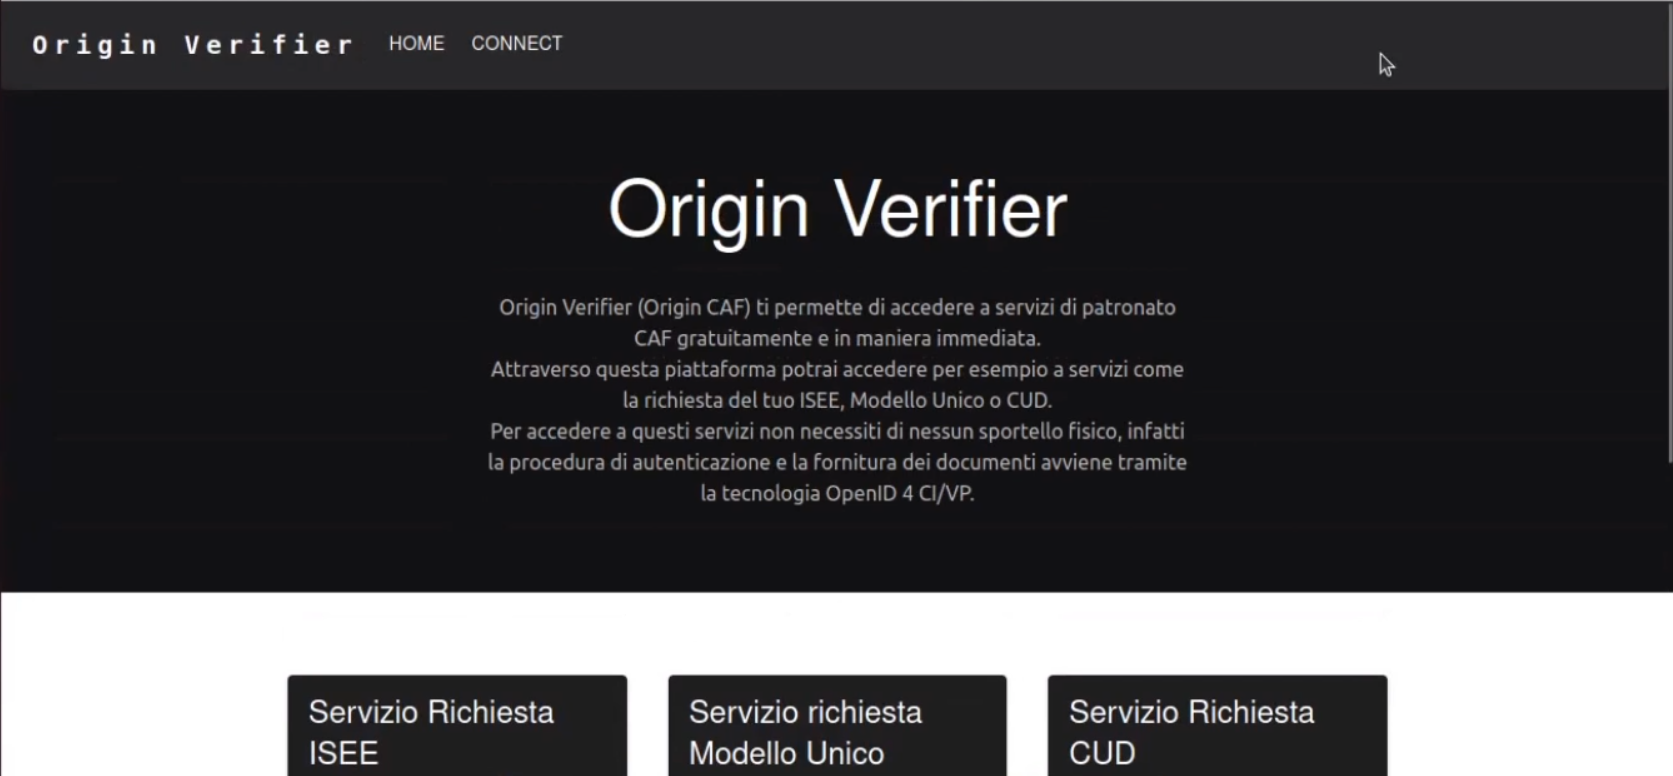
\includegraphics[scale = 0.2]{./res/img/verifier/homeverifier.png}
    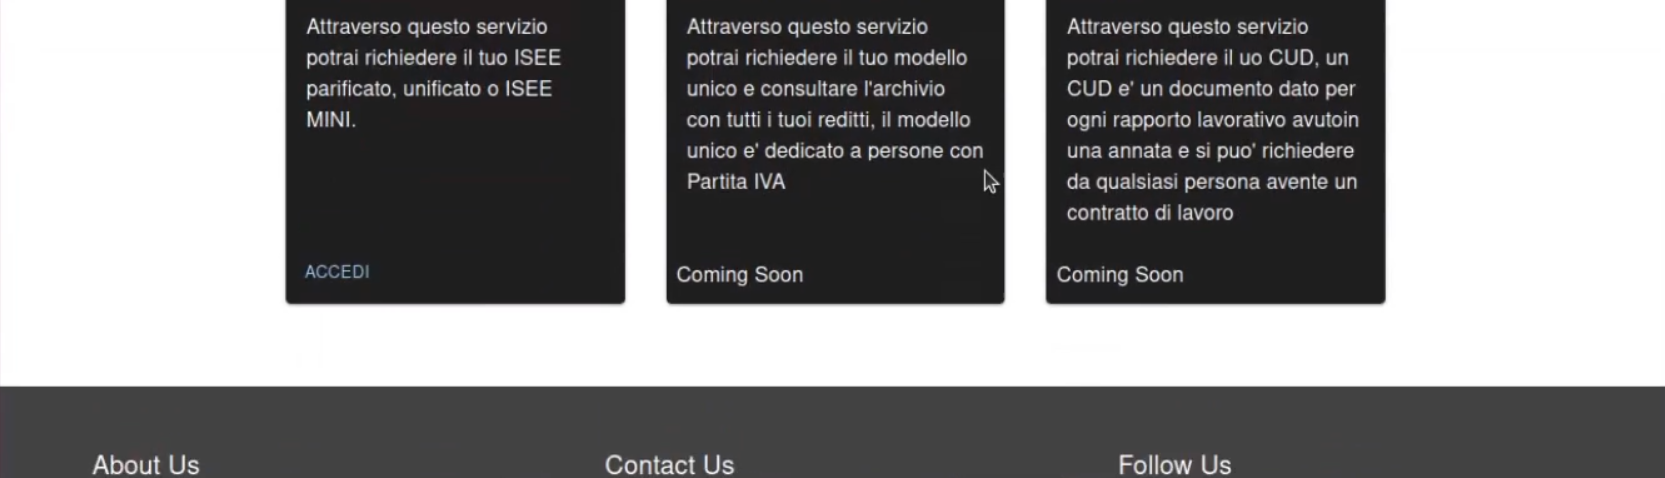
\includegraphics[scale = 0.2]{./res/img/verifier/homeverifier2.png}
    \end{center}
Per accedervi però bisogna prima connettersi al proprio wallet. Per fare ciò dalla navbar bisogna cliccare il tasto "connect".\\
\begin{center}
    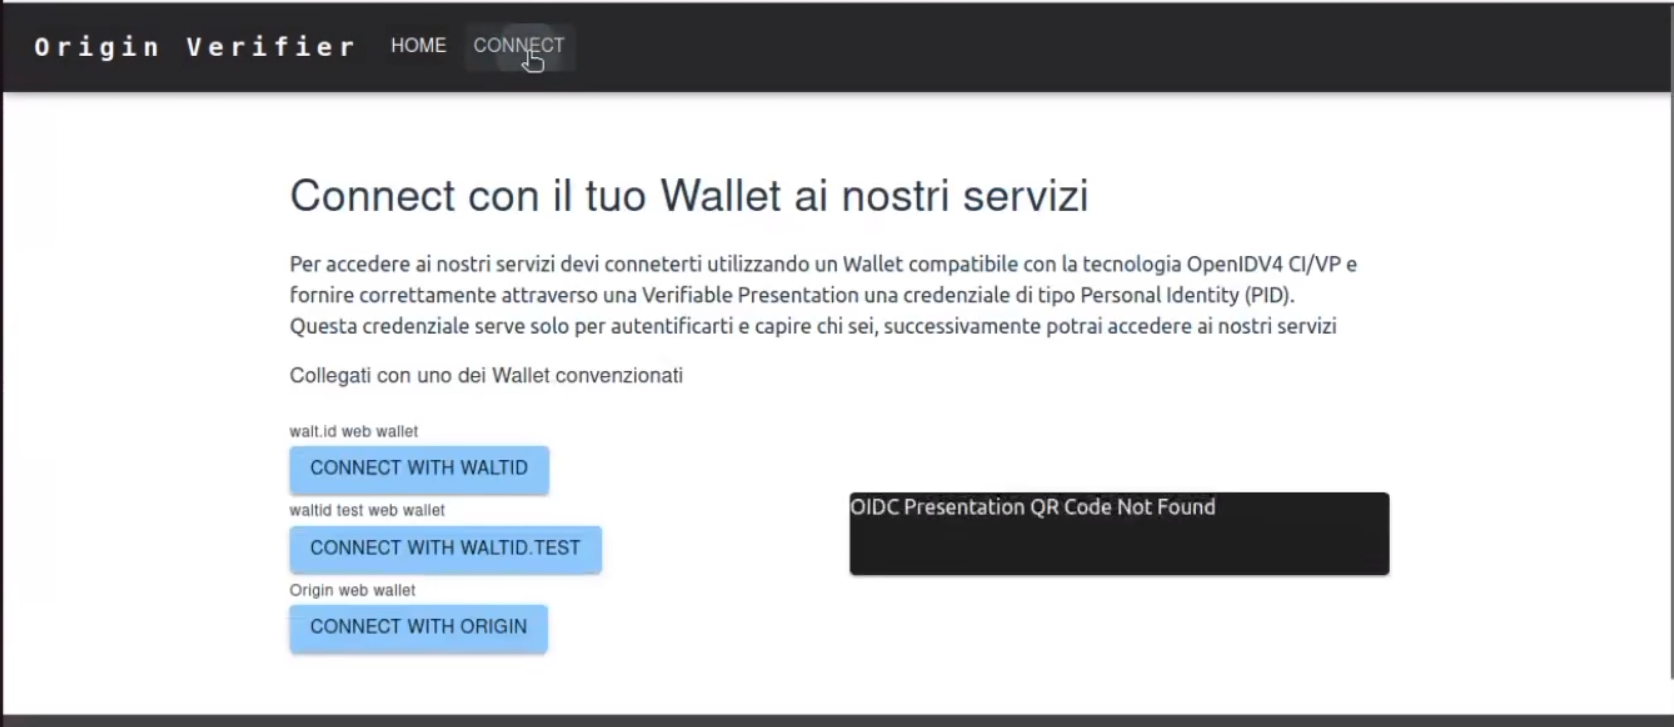
\includegraphics[scale = 0.2]{./res/img/verifier/connessione1.png}
\end{center}
il Link porterà ad una pagina dove sarà possibile eseguire il login al proprio wallet tramite un link da inserire nella sezione "Start Presentation" del mio origin Wallet. 

\begin{center}
    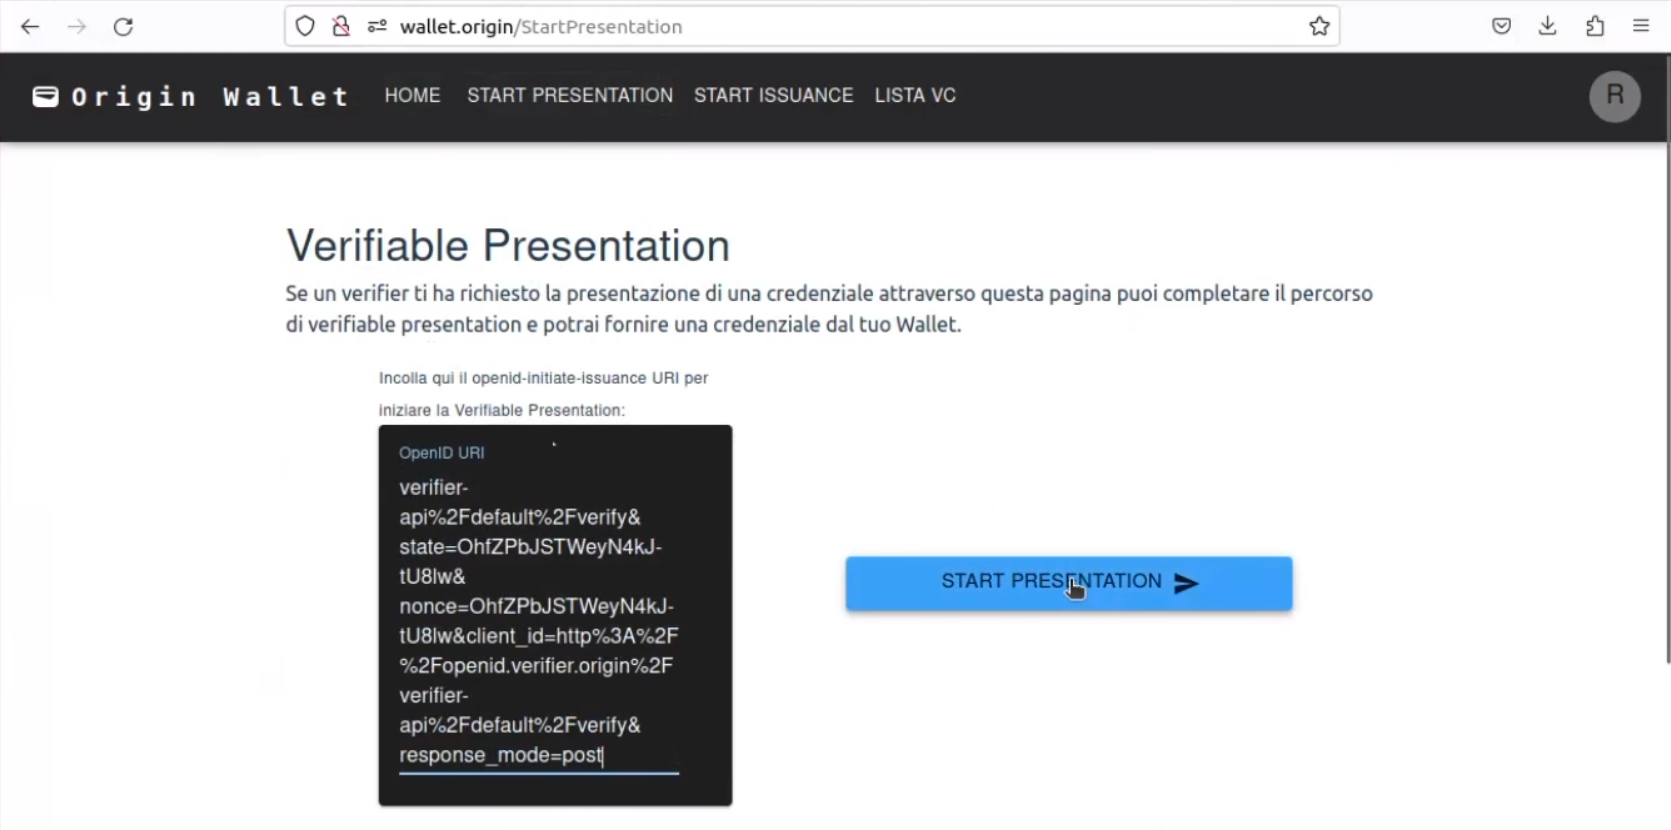
\includegraphics[scale = 0.2]{./res/img/verifier/Connessione2.png}
\end{center}

\subsection{Presentazione credenziale}
Una volta connesso il wallet si avrà a disposizione una lista di credenziali tra qui scegliere. Da notare che in questa lista non saranno presenti tutte le credenziali che sono presenti all'interno del wallet dell'utente, ma soltanto quelle compatibili e accettate dal verifier ovvero dal servizio di verifica.\\
\begin{center}
    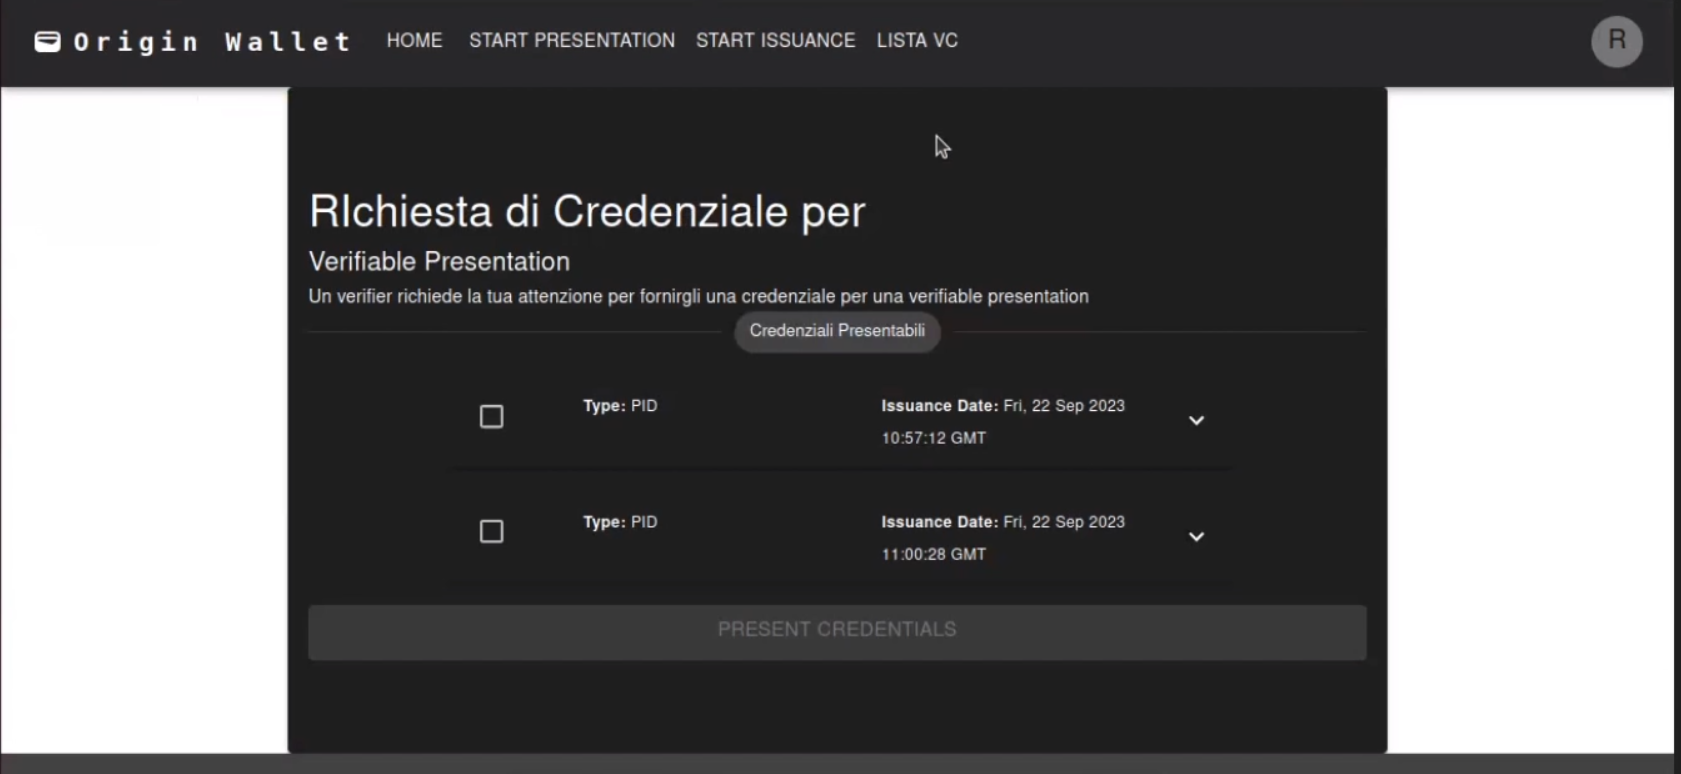
\includegraphics[scale = 0.2]{./res/img/verifier/presentazione1.png}
\end{center}
Selezionate le credenziali e cliccato il pulsante "present credentials" si verrà reindirizzati al verifier. \\
\begin{center}
    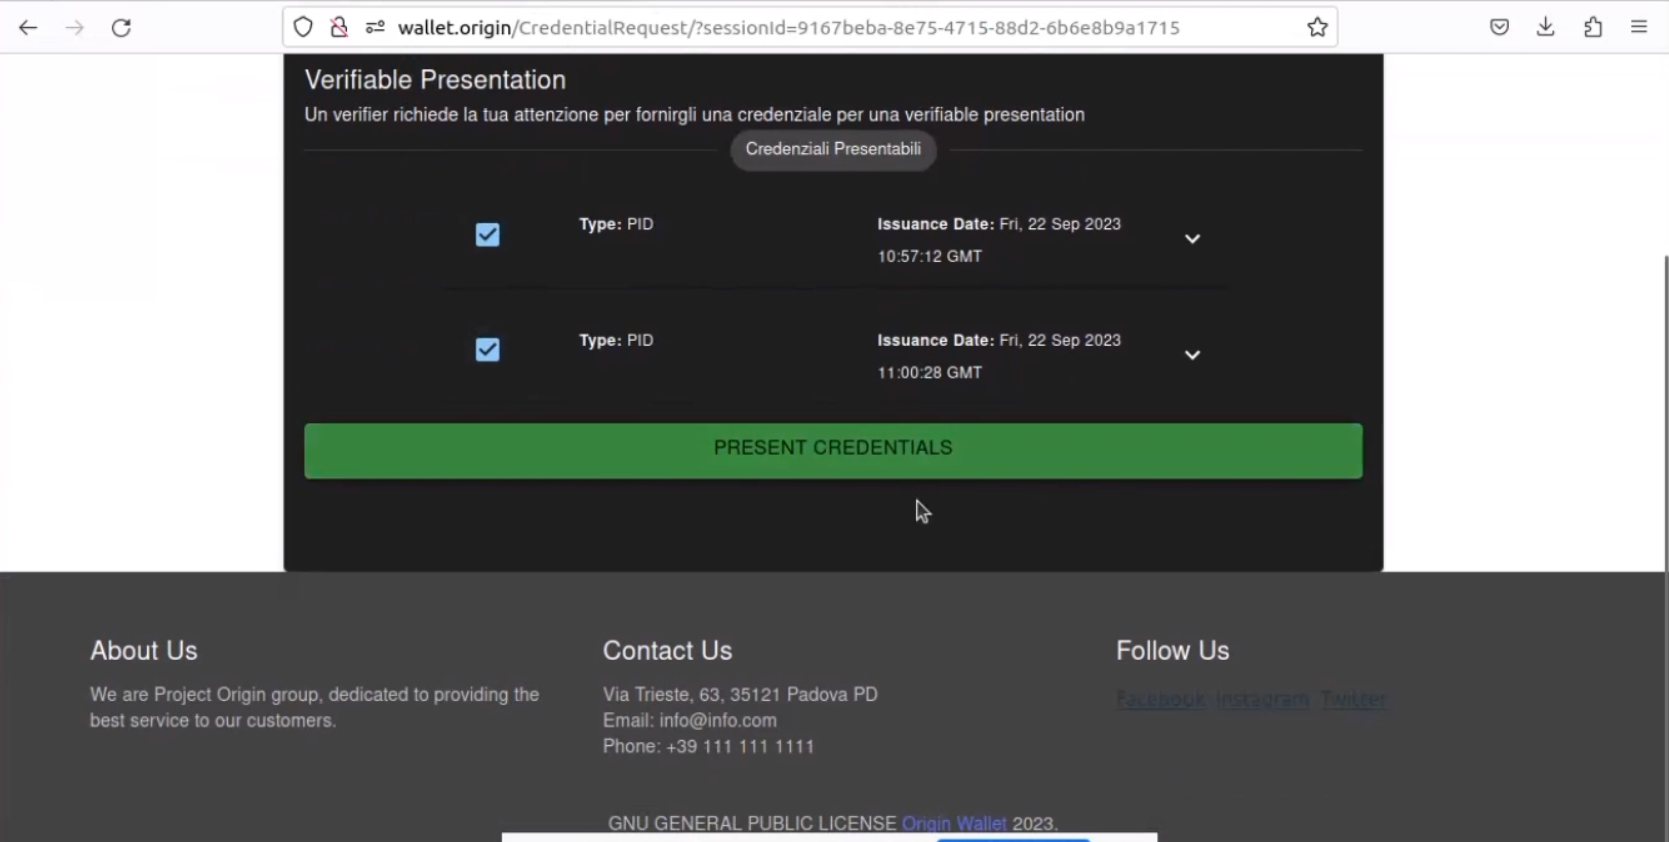
\includegraphics[scale = 0.2]{./res/img/verifier/presentazione2.png}
\end{center}
Ci verrà ora mostrata una schermata di esito della presentazione con i dati di chi ha presentato la credenziale e le informazioni. Sono inoltre mostrati a scermo gli esiti della verifica della credenziale secondo determinate Policy. \\
\begin{center}
    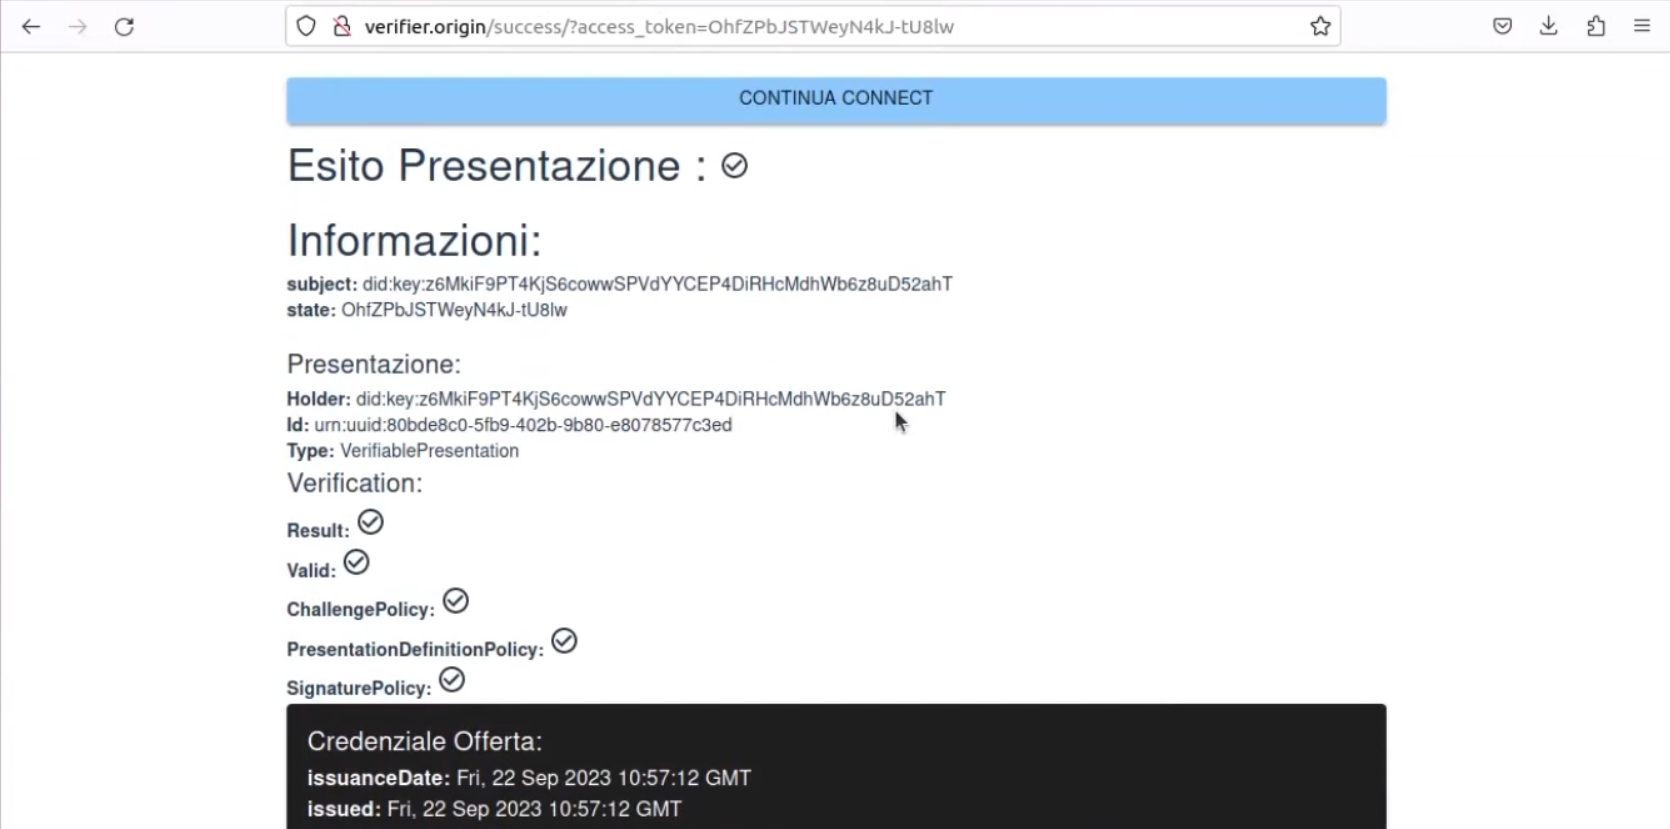
\includegraphics[scale = 0.2]{./res/img/verifier/esito.png}
\end{center}

\subsection{Accesso ai servizi}
Se dalla schermata "Home" provassimo ad accedere ad un servizio offerto da verifier come in questo caso Servizio isee e l'untente non avesse ancora eseguito la connessione al Wallet e verificato la credenziale necessaria per accedervi, verrà mostrato a schermo un messaggio di errore che cita l'invalidità del token.

\begin{center}
    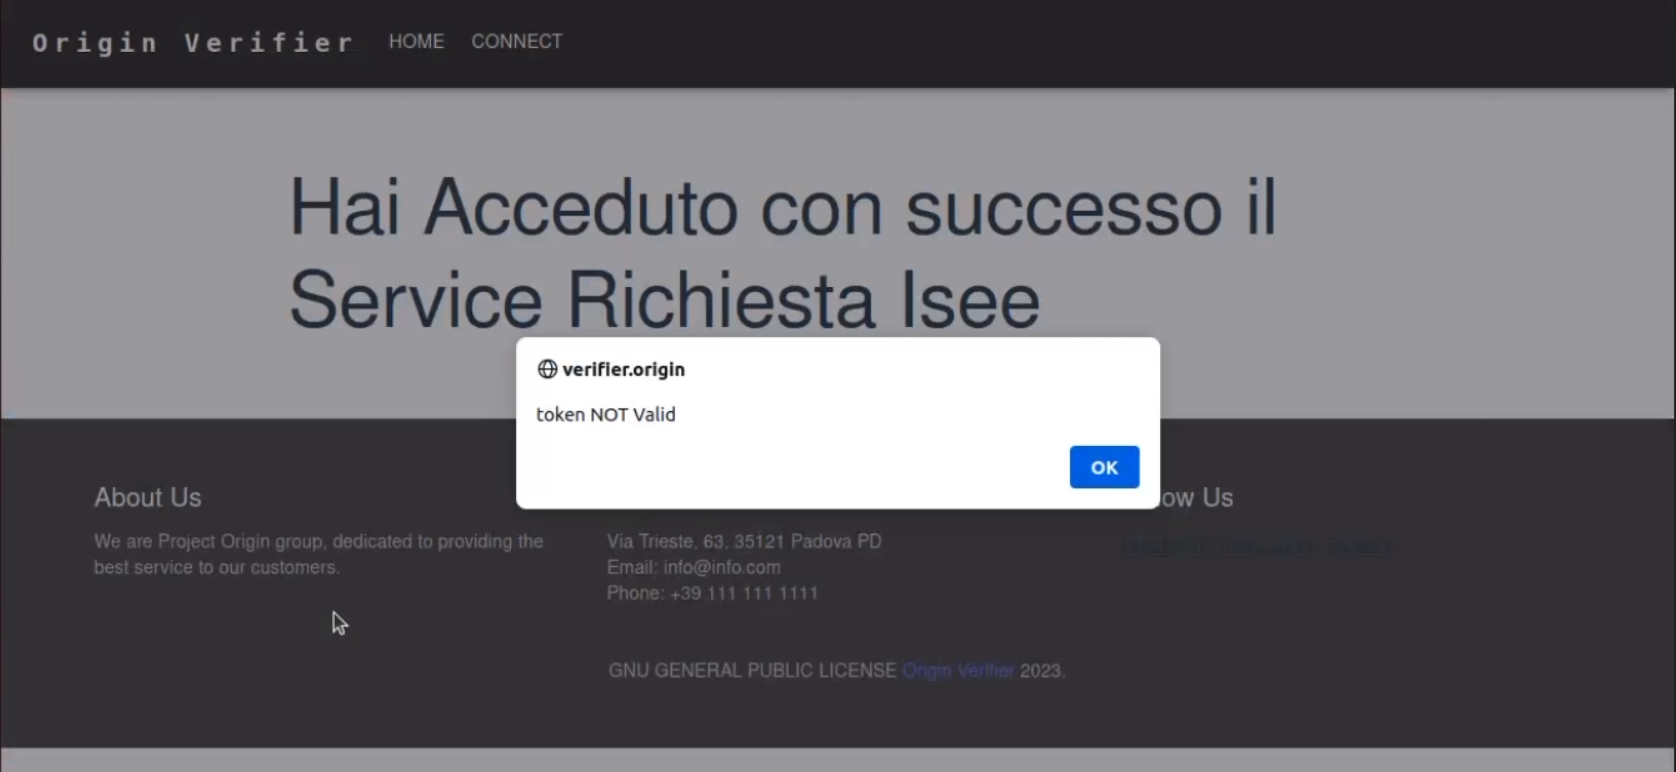
\includegraphics[scale = 0.2]{./res/img/verifier/tokenNONvalido.png}
\end{center}

Se l'utente avesse esegito la  "Presentazione Credenziale" descritta nella sezione precedente può accedere al "Servizio isee" offerto avendo un messaggio di corretto token a disposizione e accedendo correttamente al servizio.\\

\begin{center}
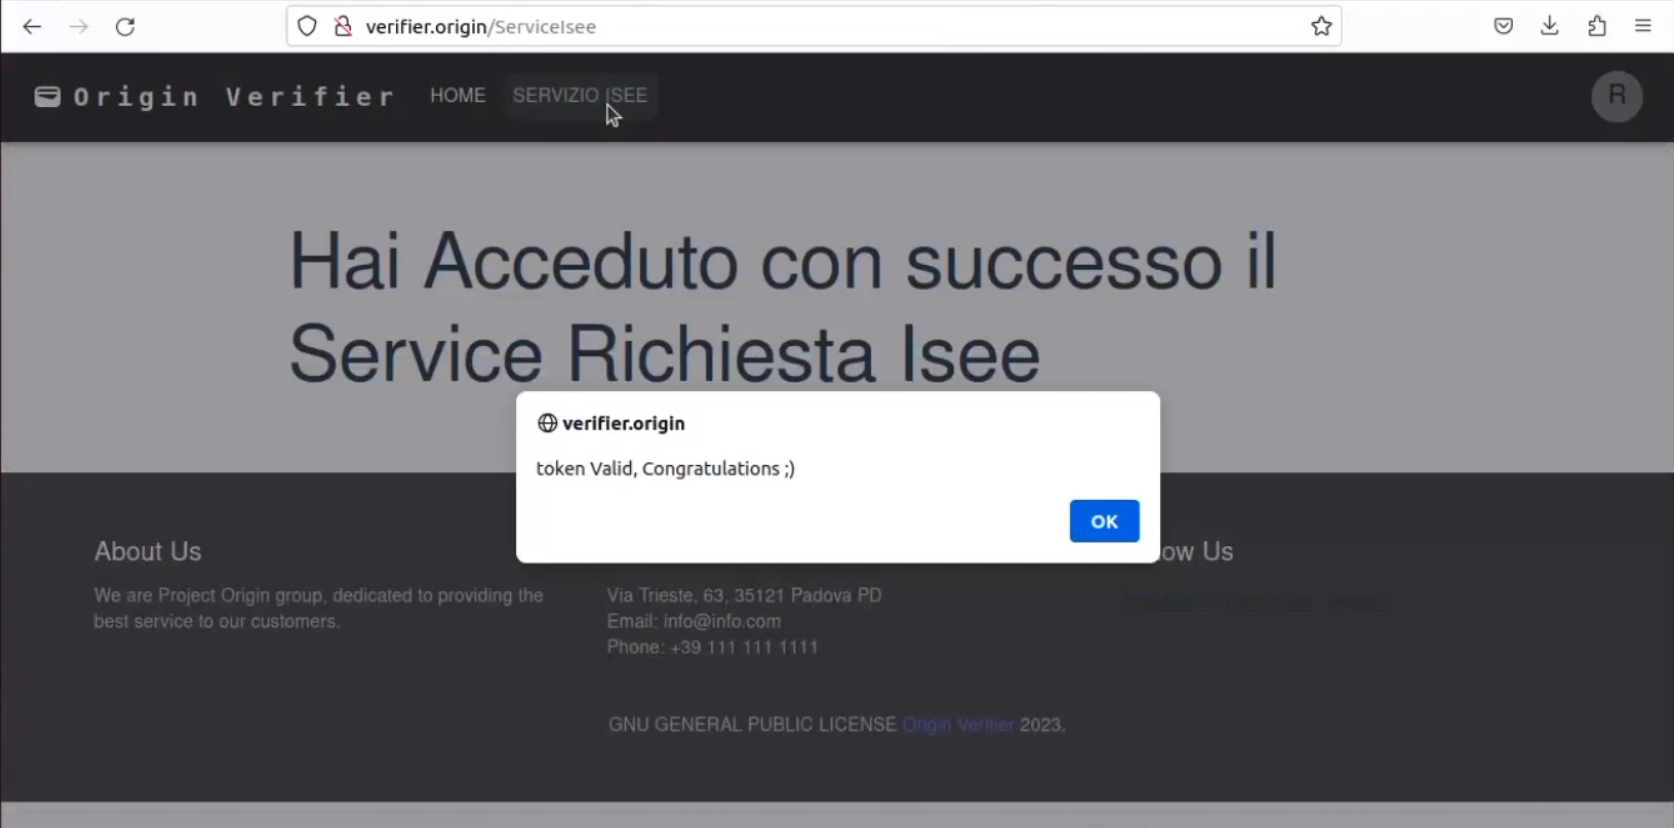
\includegraphics[scale = 0.2]{./res/img/verifier/tokenvalido.png}
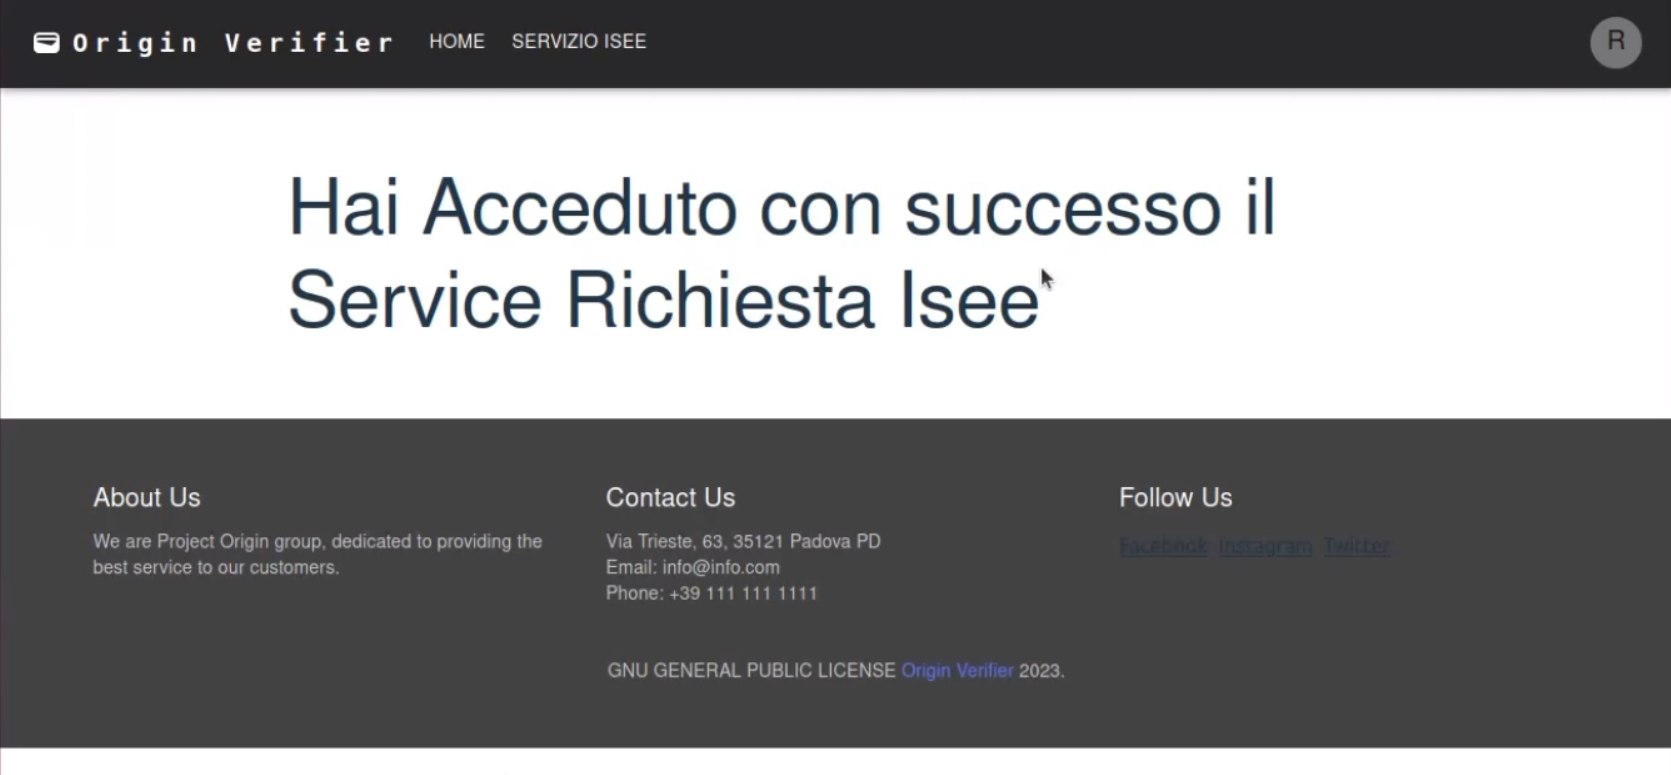
\includegraphics[scale = 0.2]{./res/img/verifier/accessoservizio.png}
\end{center}